\documentclass[a4j]{jarticle}

\usepackage[dvipdfmx]{graphicx}
\usepackage{url}
\usepackage{here}
%\usepackage{listings}
\usepackage{amsmath,amssymb}
\usepackage[dvipdfmx]{color}

\setlength{\headsep}{-5mm}
\setlength{\oddsidemargin}{0mm}
\setlength{\textwidth}{165mm}
\setlength{\textheight}{230mm}
\setlength{\footskip}{20mm}

\title{
\vspace{30mm}
{\bf 子育て支援システム}
\\
\vspace{5mm}
{\bf 内部設計書v1\\
}
\vspace{120mm}
}

\author{
\vspace{5mm}
チーム名 007\\
\vspace{5mm}
}


\begin{document}
\maketitle
\tableofcontents
\newpage

\section{開発環境}
本章では、システムを開発する際に必要となる環境を示しています。

\subsection{Androidアプリの開発環境}
Androidアプリの開発環境を表\ref{Application_Development_Environment}に示します。

\begin{table}[H]
    \caption{Androidアプリの開発環境}
    \label{Application_Development_Environment}
    \begin{center}
        \begin{tabular}{|c||c|} \hline
            IDE & Android Studio 3.2.1 \\ \hline
            開発言語 & Java, PHP \\ \hline
            画面設計 & XML \\ \hline
            バージョン管理 & GitHub \\ \hline
        \end{tabular}
    \end{center}
\end{table}

\subsection{サーバの開発環境}
システムで使用するサーバの開発環境を表\ref{Server_Development_Environment}に示します。
\begin{table}[H]
    \caption{サーバの開発環境}
    \label{Server_Development_Environment}
    \begin{center}
        \begin{tabular}{|c||c|} \hline
            OS & CentOS 7.5.1804 \\ \hline
            サーバソフトウェア & Apache 2.4.6 \\ \hline
            データベース & mysql 14.14 \\ \hline
            CPU & Intel Corei7-3930K \\ \hline
            RAM & 32GB \\ \hline
            ROM & 500GB \\ \hline
        \end{tabular}
    \end{center}
\end{table}


\section{動作環境}
本章では、システムを動作させる際に必要となる環境を示しています。

表\ref{Operationg_Environment}に動作環境の情報を示します。

\begin{table}[H]
    \caption{動作環境}
    \label{Operationg_Environment}
    \begin{center}
        \begin{tabular}{|c||c|} \hline
            OS & Android4.4 以上 9.0以下 \\ \hline
            画面 & 高解像度(hdpi) \\ \hline
            必要機能 & カメラ \\ \hline
            通信 & 3G/4G(LTE)またはWi-Fiによるインターネット接続 \\ \hline
            CPU & 1GHz以上 \\ \hline
            RAM & 2GB以上 \\ \hline

        \end{tabular}
    \end{center}
\end{table}

\section{コーディング規約}
本章では、本システムを開発する際のコーディング規約を示します。

\subsection{命名規則}
\begin{itemize}
  %スネーク記法のほうが良ければスネーク記法にしましょ(例:setting_account)
  \item クラス名・モジュール名
  %アッパーキャメルケース表記で命名を行います。
  \begin{itemize}
    \item 2つ以上の英単語を使用します。
    \item 単語の頭文字は全て大文字を使用します。
    \item 名称は英字のみを使用し、意味のあるものを用います。
  \end{itemize}
  (例:SettingAccount)

  \item メソッド名・変数名
  %ローワーキャメルケース表記で命名を行います。
  \begin{itemize}
    \item 2つ以上の英単語を使用します。
    \item 名称の頭文字は小文字、後続する単語の頭文字は大文字を使用します。
    \item 名称は英字のみを使用し、意味のあるものを用います。
  \end{itemize}
  (例:getStatus)

  \item 定数
  \begin{itemize}
    \item 全ての文字を大文字で表記します。
    \item 2つ以上の単語を用いる場合は、単語と単語を‘\_’で区切ります。
  \end{itemize}
  (例:ERRAND\_ID)
  %errand -> おつかいの意味
\end{itemize}

\subsection{コーディングスタイル}

\begin{itemize}
  \item インデント
  \begin{itemize}
    \item インデントはTAB文字、または半角スペース4文字を使用します。
  \end{itemize}

  \item 括弧
  \begin{itemize}
    \item 中括弧は改行して開始します。
    \item 小括弧の前後にはスペースを使用しない。
  \end{itemize}

  \item 演算子
  \begin{itemize}
    \item 演算子の前後には半角スペースを一文字分使用します。
  \end{itemize}

  %\item 文字コード
\end{itemize}

\section{モジュール設計書}
モジュール構成において各図形が何を意味するか図\ref{sample}に示してあります。


\begin{figure}[H]
    \begin{center}
    \resizebox{8cm}{!}{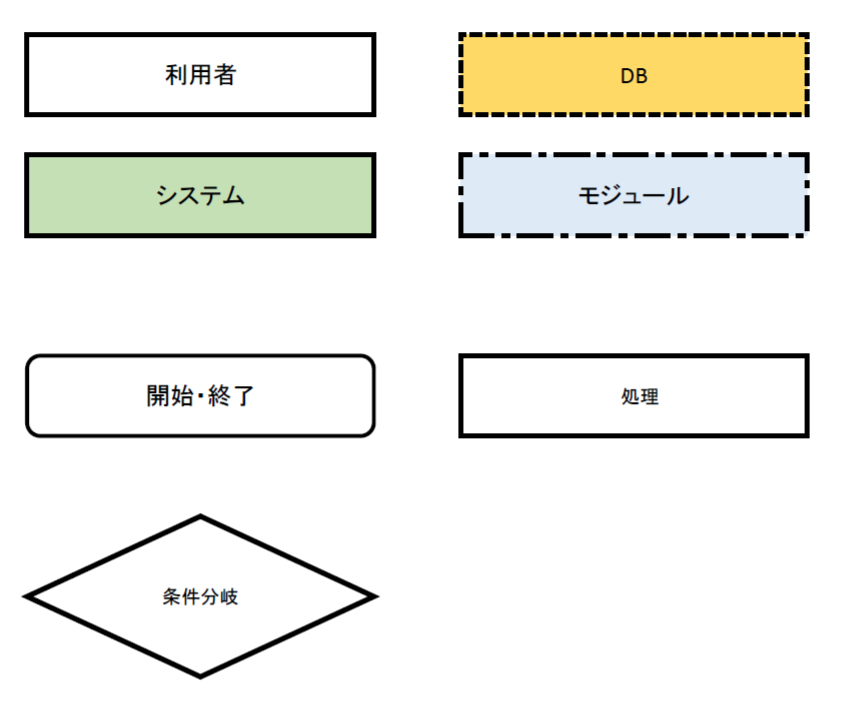
\includegraphics {sample.png}}
    \caption {見本のイメージ}
    \label{sample}
    \end{center}
\end{figure}

図\ref{sample}より、無色の図が「利用者側の操作」、緑色の図が「システム側の動作」、点線かつ黄色の図が「データベース側の動作」、点線かつ水色の図が「モジュール」を意味します。角の丸い四角形は「各モジュールの開始時・終了時の処理」、四角形は「各モジュールの処理内容」、ひし形は「条件分岐」を意味します。図及び文章中の【】はボタンを示しています。

\subsection{機能選択と初期設定}
\subsubsection{機能選択モジュール\label{機能選択}}
\begin{figure}[H]
    \begin{center}
    \resizebox{16.5cm}{!}{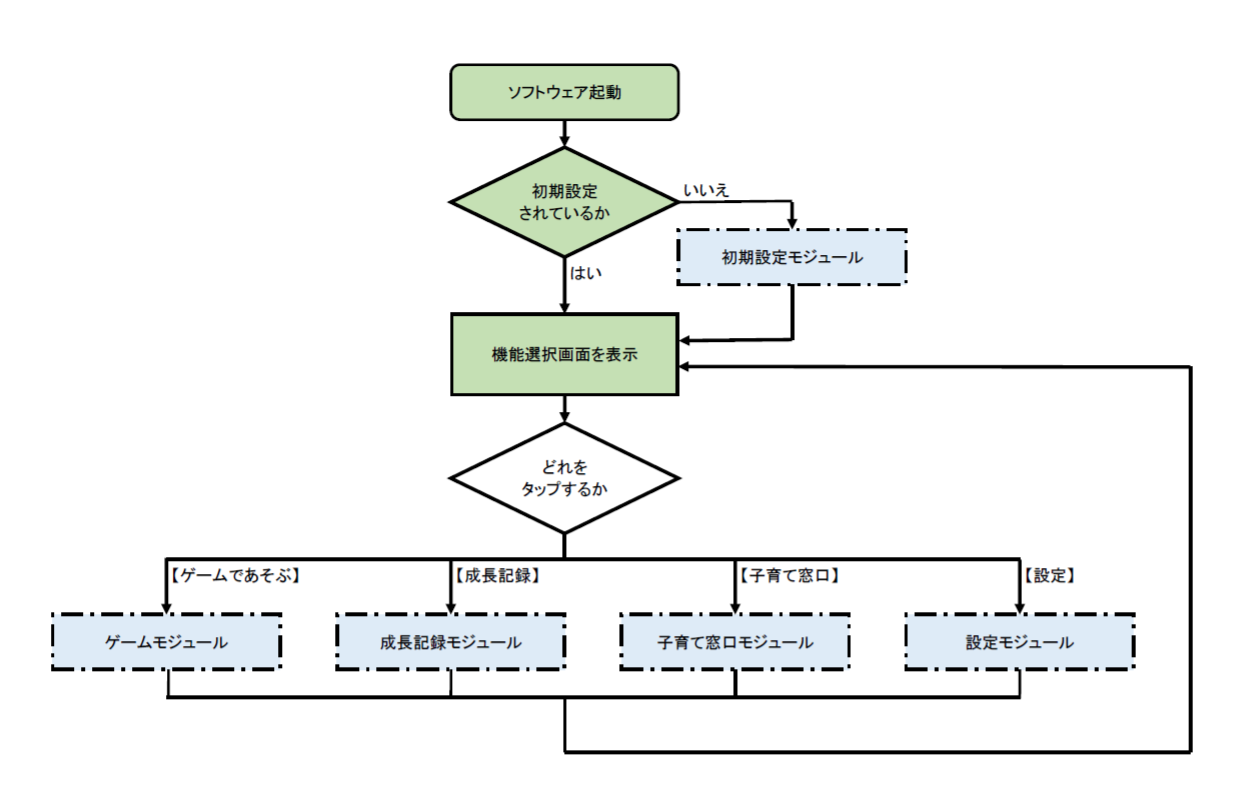
\includegraphics {functionselection.png}}
    \caption {機能選択モジュールのフローチャート}
    \label{functionselection}
    \end{center}
\end{figure}

\subsubsection*{概要}
図\ref{functionselection}は、本システムを起動してから各機能選択を行うまでのシステムの流れを示しています。

\subsubsection*{処理フロー}
\begin{itemize}
\item 本システムを起動した際に、初期設定が行われていればそのまま機能選択画面を表示させます。初期設定が行われていない場合は初期設定モジュール(第\ref{初期設定}節)を呼び出します。

\item 【ゲームであそぶ】をタップすることでゲームモジュール(第\ref{ゲーム}節)を呼び出します。

\item 【成長記録】をタップすることで成長記録モジュール(第\ref{grow}節)を呼び出します。

\item 【子育て窓口】をタップすることで子育て窓口モジュール(第\ref{子育て窓口モジュール}節)を呼び出します。

\item 【設定】をタップすることで設定モジュール(第\ref{設定}節)を呼び出します。

\item 機能選択画面から呼び出される各モジュールにおいて【もどる】をタップすることで、機能選択画面(本節)に遷移します。
\end{itemize}

\begin{figure}[H]
\subsubsection{初期設定モジュール\label{初期設定}}
    \begin{center}
    \resizebox{16.5cm}{!}{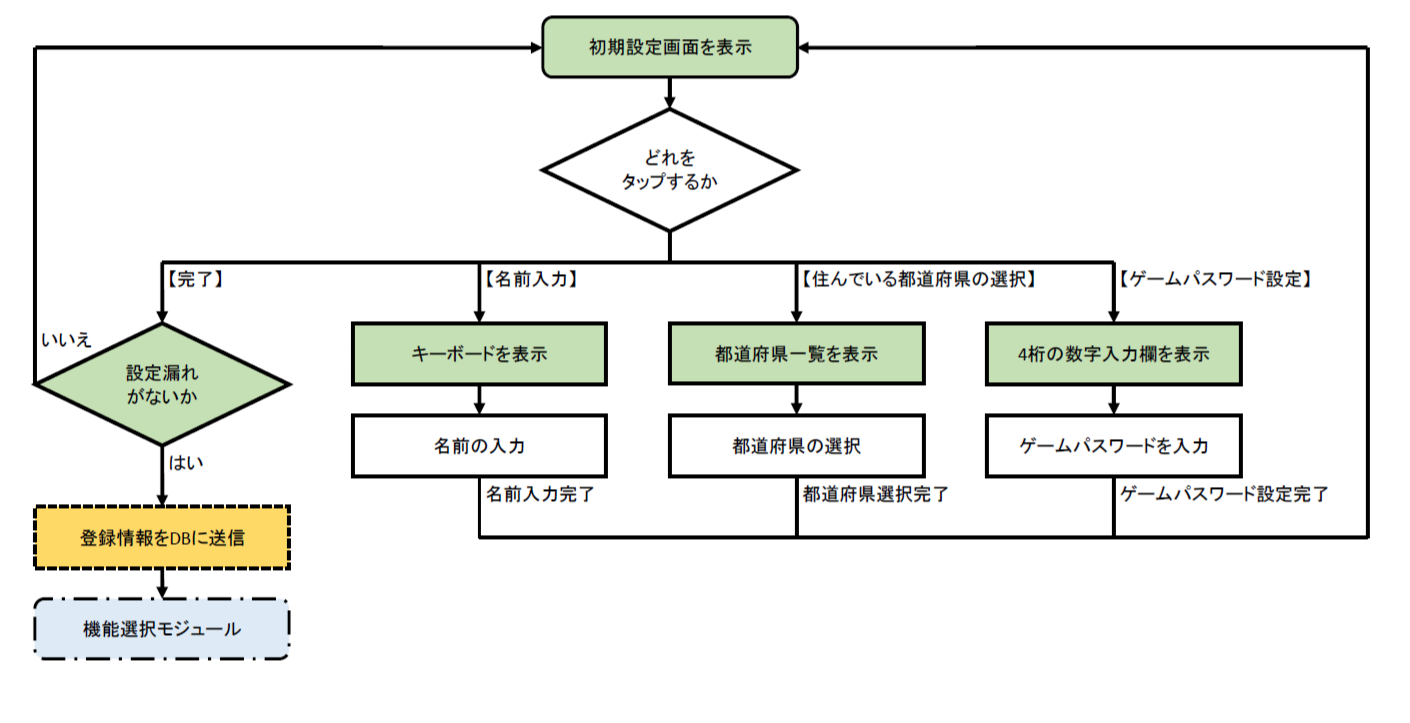
\includegraphics {initialsetting.png}}
    \caption {初期設定モジュールのフローチャート}
    \label{initialsetting}
    \end{center}
\end{figure}


\subsubsection*{概要}
図\ref{initialsetting}は、本システムを初めて利用する場合の初期設定機能のシステムの流れを示しています。


\subsubsection*{処理フロー}
\begin{itemize}
\item 【名前(ニックネーム)の入力欄】をタップすることで画面下にキーボードが表示され、名前入力を行えるようになります。

\item 【居住地域の選択欄の矩形領域】をタップすることで47都道府県をタップして選択できるドロップダウンリストを「都道府県コード順」に表示させ、住んでいる地域設定が行えるようになります。

\item 【ゲームのパスワードの入力欄】をタップすることでキーボードを表示させ、ゲーム画面から機能選択画面に戻るためのパスワードとして、4桁の数字が入力できるようになります。

\item 【完了】をタップすることで初期設定が全て行われているか判定を行い、設定漏れがなければデータベースに初期設定情報を登録して機能選択モジュール(第\ref{機能選択}節)を呼び出します。設定漏れが見つかれば再び初期設定画面(本節)に遷移し、設定漏れを埋めることになります。
\end{itemize}

\newpage


\subsection{ゲーム機能}
\subsubsection{ゲームモジュール\label{ゲーム}}
\begin{figure}[H]
    \begin{center}
    \resizebox{16.5cm}{!}{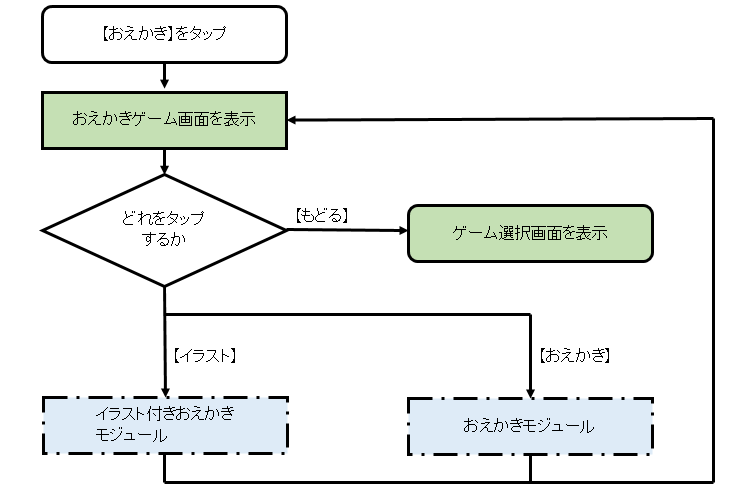
\includegraphics {game.png}}
    \caption {ゲームモジュールのフローチャート}
    \label{game}
    \end{center}
\end{figure}

\subsubsection*{概要}
 図\ref{game}は、利用者が行うゲーム選択のシステムの流れを示しています。

\subsubsection*{処理フロー}
\begin{itemize}
\item 【おえかき】をタップすることでおえかき選択モジュール(第\ref{おえかき選択}節)を呼び出します。
\item 【おつかい】をタップすることでおつかいモジュール(第\ref{おつかい}節)を呼び出します。
\item 【もどる】をタップすることで機能選択画面(第\ref{機能選択}節)に遷移します。
\end{itemize}

\newpage

\subsubsection{おえかき選択モジュール\label{おえかき選択}}
\begin{figure}[H]
    \begin{center}
    \resizebox{16.5cm}{!}{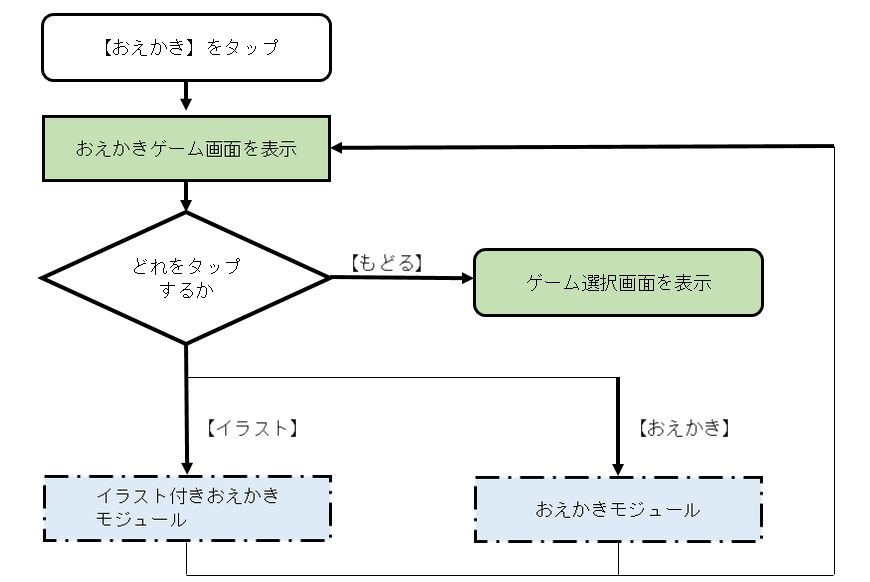
\includegraphics {oekaki.png}}
    \caption {おえかき選択モジュールのフローチャート}
    \label{oekaki}
    \end{center}
\end{figure}

\subsubsection*{概要}
 図\ref{oekaki}は、おえかきゲームの種類を選択するシステムの流れを示しています。

\subsubsection*{処理フロー}
\begin{itemize}
\item 【イラスト】をタップすることでイラスト付きおえかきモジュール(第\ref{イラスト}節)を呼び出します。
\item 【おえかき】をタップすことでおえかきモジュール(第\ref{おえかき}節)を呼び出します。
\item 【もどる】をタップすることでゲーム選択画面(第\ref{ゲーム}節)に遷移します。
\end{itemize}

\newpage
\subsubsection{おえかきモジュール\label{おえかき}}
\begin{figure}[H]
    \begin{center}
    \resizebox{16.5cm}{!}{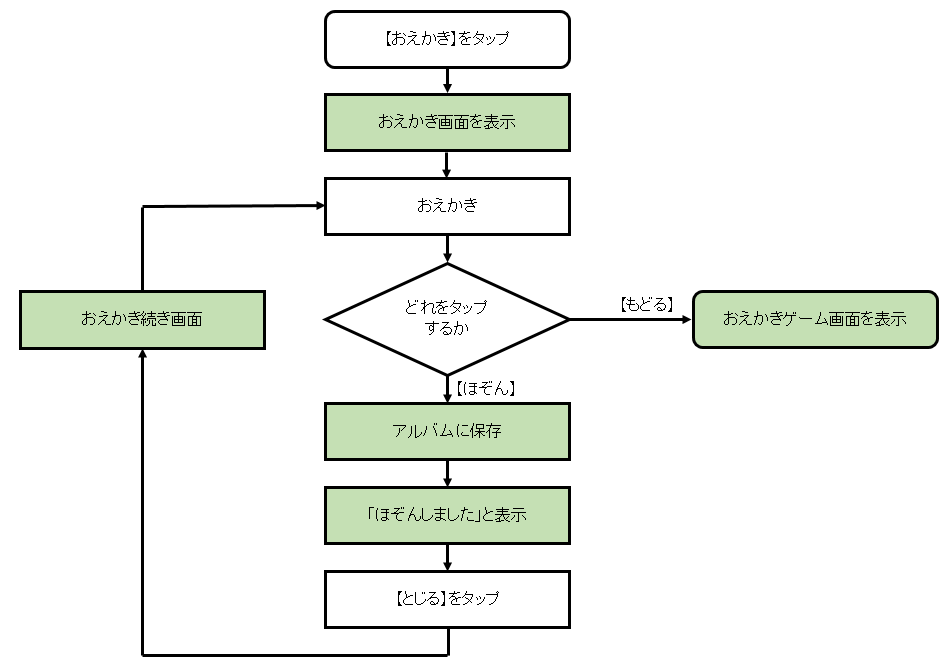
\includegraphics {oekaki2.png}}
    \caption {おえかきモジュールのフローチャート}
    \label{oekaki2}
    \end{center}
\end{figure}

\subsubsection*{概要}
図\ref{oekaki2}は、利用者が実際におえかきゲームで遊ぶ際のシステムの流れを示しています。

\subsubsection*{処理フロー}
\begin{itemize}
\item 【イラスト】をタップすることでおえかきをするためのペンやペンの太さ、消しゴム、色の種類を変更できます。
\item 【ほぞん】をタップすことで利用者の描いたおえかきが成長記録のアルバムに保存されます。
\item 「ほぞんしました」と表示された画面の【とじる】をタップするとおえかきの続き画面(本節)に遷移します。 
\item 【もどる】をタップすることでおえかき選択画面(第\ref{おえかき選択}節)に遷移します。
\end{itemize}

\newpage
\subsubsection{イラスト付きおえかきモジュール\label{イラスト}}
\begin{figure}[H]
    \begin{center}
    \resizebox{16.5cm}{!}{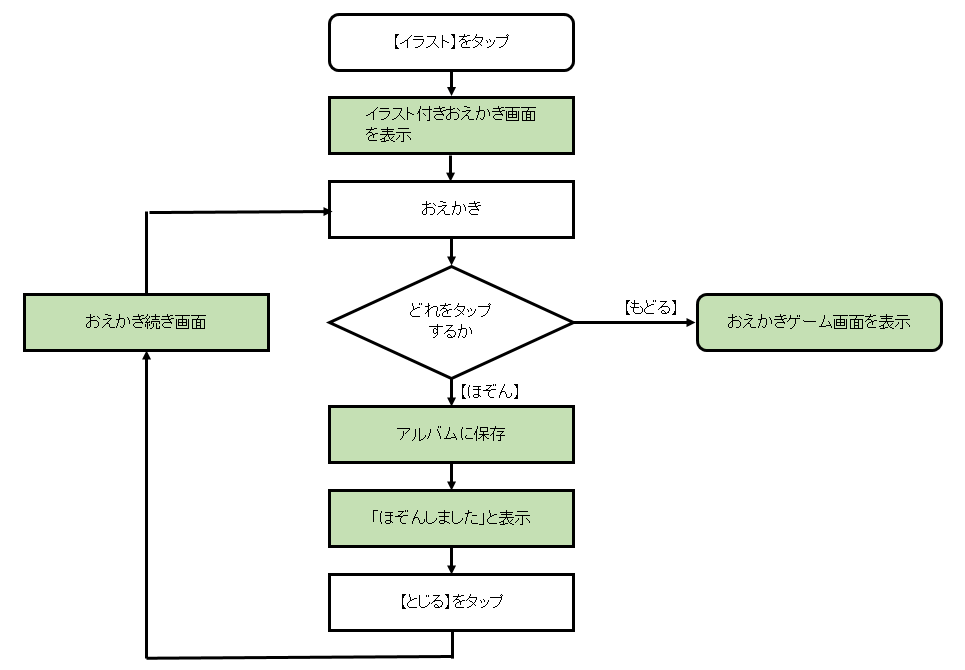
\includegraphics {illustration.png}}
    \caption {イラスト付きおえかきモジュールのフローチャート}
    \label{illustration}
    \end{center}
\end{figure}

\subsubsection*{概要}
図\ref{illustration}は、利用者が実際にイラスト付きおえかきゲームで遊ぶ際のシステムの流れを示しています。

\subsubsection*{処理フロー}
\begin{itemize}
\item 【イラスト】をタップすることでおえかきをするためのペンやペンの太さ、消しゴム、色の種類を変更できます。
\item 【ほぞん】をタップすことで利用者の描いたおえかきが成長記録のアルバムに保存されます。
\item 「ほぞんしました」と表示された画面の【とじる】をタップするとおえかきの続き画面(本節)に遷移します。
\item 【もどる】をタップすることでおえかき選択画面(第\ref{おえかき選択}節)に遷移します。
\end{itemize}


\newpage

\subsubsection{おつかい画面モジュール\label{おつかい}}
\begin{figure}[H]
    \begin{center}
    \resizebox{16.5cm}{!}{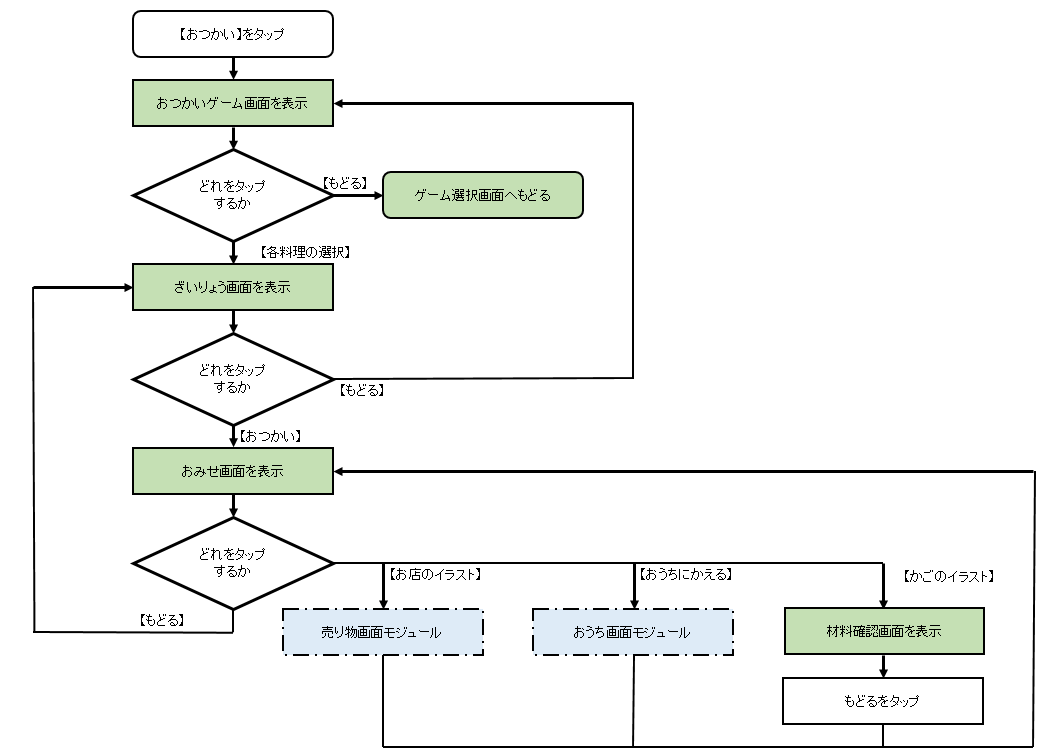
\includegraphics {otukai.png}}
    \caption {おつかい画面モジュールのフローチャート}
    \label{otukai}
    \end{center}
\end{figure}

\subsubsection*{概要}
図\ref{otukai}は、利用者が実際におつかいゲームで遊ぶ際のシステムの流れを示しています。

\subsubsection*{処理フロー}
\begin{itemize}
\item 【もどる】をタップすることでゲーム選択画面(第\ref{ゲーム}節)に遷移します。
\item 【料理のイラスト】をタップすることで選択した料理の材料画面を表示します。
\item 材料画面の【おつかい】をタップするとおみせ画面を表示し、【もどる】をタップするとおつかいゲーム画面(本節)を表示します。
\item 【お店のイラスト】をタップすることで売り物画面モジュール(第\ref{売り物}節)を呼び出します。
\item 【おうちにかえる】をタップすることでおうち画面モジュール(第\ref{おうち}節)を呼び出します。
\item 【かごのイラスト】をタップすることで材料確認画面に遷移し持っている材料を確認できます。

\end{itemize}


\newpage
\subsubsection{売り物モジュール\label{売り物}}
\begin{figure}[H]
    \begin{center}
    \resizebox{16.5cm}{!}{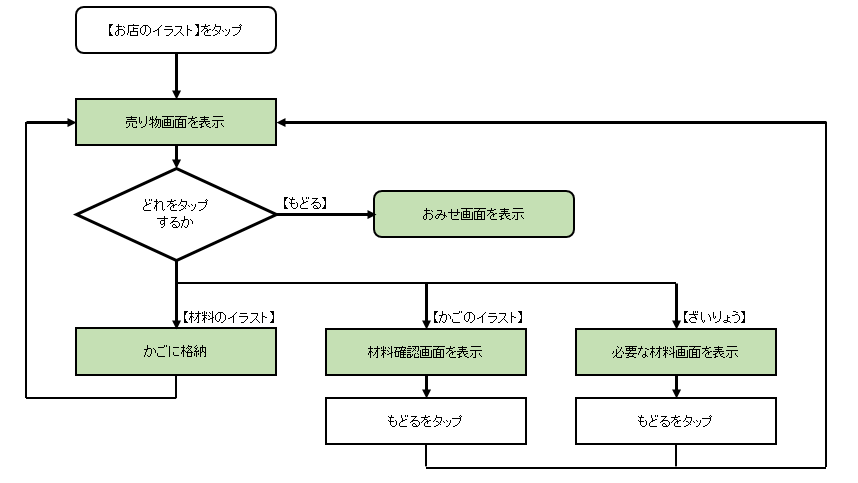
\includegraphics {urimono.png}}
    \caption {売り物モジュールのフローチャート}
    \label{urimono}
    \end{center}
\end{figure}

\subsubsection*{概要}
図\ref{urimono}はおつかいゲームで必要な材料を買う際のシステムの流れを示しています。

\subsubsection*{処理フロー}
\begin{itemize}
\item 【もどる】をタップすることでおみせ画面(本節)に遷移します。
\item 【材料のイラスト】をタップすることでかごにタップした材料が格納されます。
\item 【かごのイラスト】をタップすることで材料確認画面に遷移し持っている材料を確認できます。
\item 【ざいりょう】をタップすることで料理に必要な材料を表示します。
\item 材料確認画面と必要な材料画面の【もどる】をタップすることで売り物画面(本節)に遷移します。
\end{itemize}

\newpage
\subsubsection{おうちモジュール\label{おうち}}
\begin{figure}[H]
    \begin{center}
    \resizebox{9cm}{!}{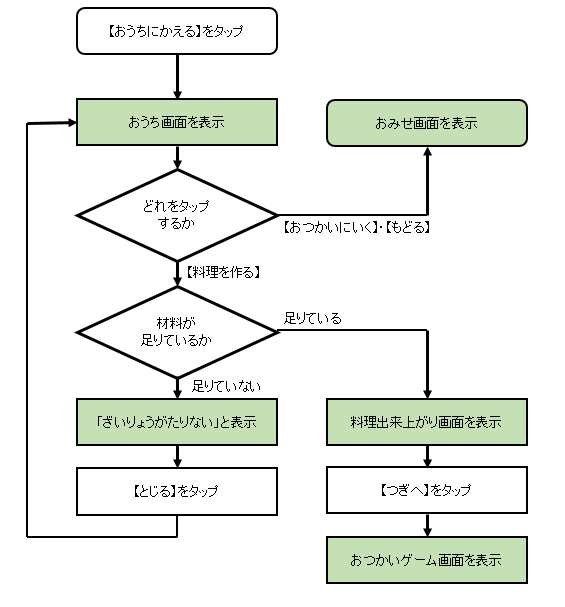
\includegraphics {outi.png}}
    \caption {おうちモジュールのフローチャート}
    \label{outi}
    \end{center}
\end{figure}

\subsubsection*{概要}
図\ref{outi}は、おつかい画面で選択した料理を持っている材料で作るまでのシステムの流れを示しています。

\subsubsection*{処理フロー}
\begin{itemize}
\item 【おつかいにいく】・【もどる】をタップすることでおみせ画面(第\ref{売り物}節)に遷移します。
\item 【料理を作る】をタップすると材料が足りている場合と足りてない場合に分岐します。足りている場合は出来上がり画面を表示し、足りてない場合は「ざいりょうがたりない」と表示します。
\item 足りている時に表示された画面の【つぎへ】をタップすることでおつかいゲーム画面(第\ref{おつかい}節)に遷移します。
\item 足りていない時に表示された画面の【とじる】をタップすることでおうち画面(本節)へ遷移します。
\end{itemize}


\subsection{成長記録機能}
\subsubsection{成長記録モジュール\label{grow}}
\begin{figure}[H]
    \begin{center}
    \resizebox{16.5cm}{!}{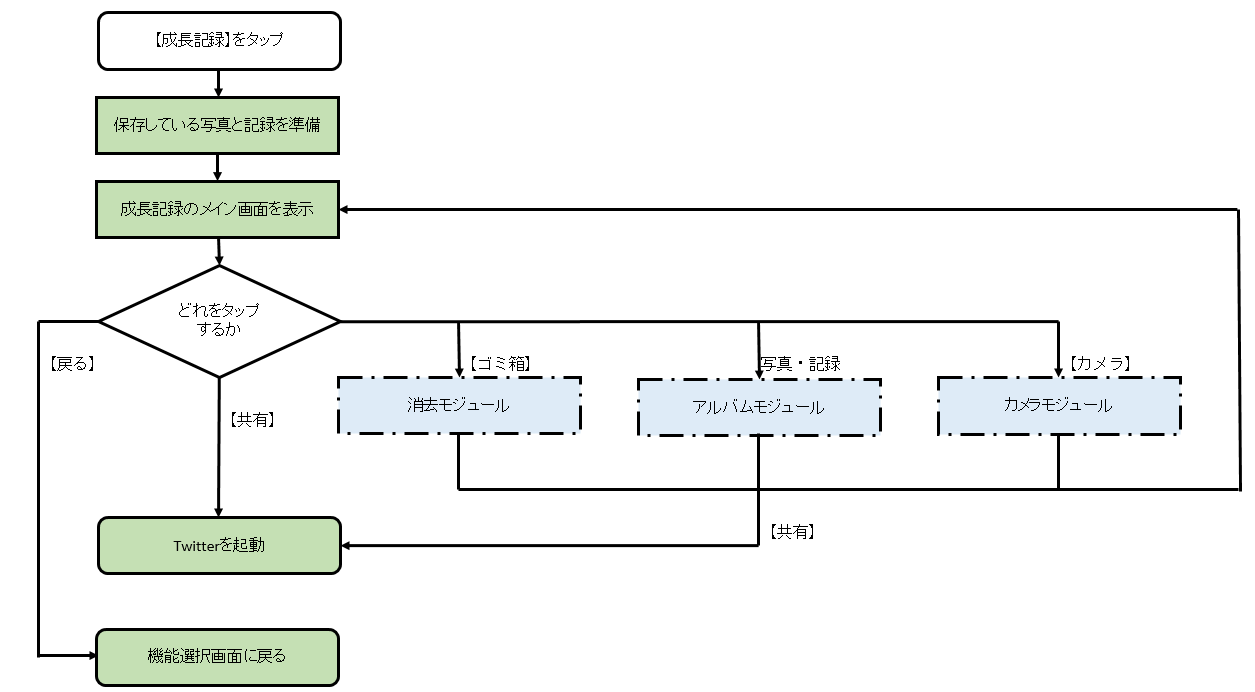
\includegraphics {growall.png}}
    \caption {成長記録モジュールのフローチャート}
    \label{growall}
    \end{center}
\end{figure}


\subsubsection*{概要}
図\ref{growall}は、成長記録機能の各サブシステムを利用するまでのシステムの流れを示しています。

\subsubsection*{処理フロー}
\begin{itemize}
\item 【ゴミ箱】をタップすることで画像削除モジュール(第\ref{Delete}節)を呼び出します。

\item 写真・記録を直接タップすることでアルバムモジュール(第\ref{Albam}節)を呼び出します。

\item 【カメラ】をタップすることでカメラモジュール(第\ref{Camera}節)を呼び出します。

\item 【共有】をタップすることで外部アプリであるTwitterを起動します。

\item 【もどる】をタップすることで機能選択画面(第\ref{機能選択}節)に遷移します。
\end{itemize}

\subsubsection{画像削除モジュール\label{Delete}}
\begin{figure}[H]
    \begin{center}
    \resizebox{10cm}{!}{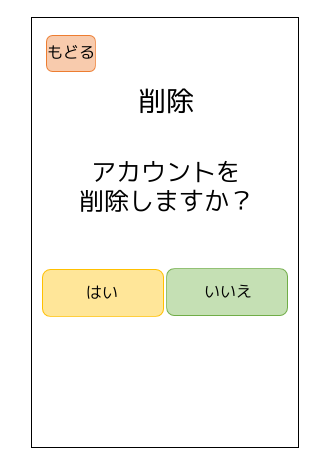
\includegraphics {delete.png}}
    \caption {画像削除モジュールのフローチャート}
    \label{delete}
    \end{center}
\end{figure}

\subsubsection*{概要}
図\ref{delete}は、利用者が不要と判断した写真やゲームの記録の削除を行う際のシステムの流れを示しています。

\subsubsection*{処理フロー}
\begin{itemize}
\item 削除したい写真や記録をタップすることでその写真や記録にチェックマークが表示されます。その後、【削除】するか【もどるボタン】を選択します。
\item 【削除】を選んだ場合確認画面が表示されます。確認画面では【はい】と【いいえ】のボタンがあります。
\item 【はい】をタップすると選択した写真や記録が削除されます。
\item 【いいえ】をタップすると削除するか戻るかを選択する画面(本節)に遷移します。
\item 【もどるボタン】をタップした場合成長記録のメイン画面(第\ref{grow}節)に遷移します。
\end{itemize}

\subsubsection{アルバムモジュール\label{Albam}}
\begin{figure}[H]
    \begin{center}
    \resizebox{16.5cm}{!}{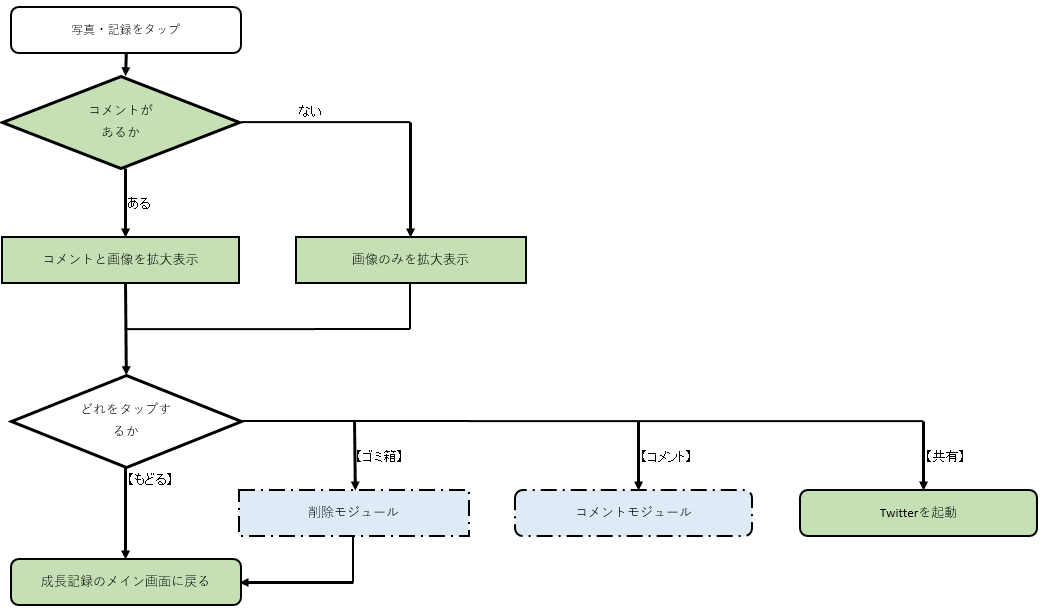
\includegraphics {albam.png}}
    \caption {アルバムモジュールのフローチャート}
    \label{albam}
    \end{center}
\end{figure}

\subsubsection*{概要}
図\ref{albam}は、利用者が閲覧したい写真や記録をタップした際のシステムの流れを示しています。

\subsubsection*{処理フロー}
\begin{itemize}
\item 写真や記録をタップした場合、それにコメントがついているかを判定します。コメントがあった場合はコメントを写真や記録と一緒に表示し、ない場合は写真や記録のみを拡大表示します。拡大表示した画面では【もどる】,【ゴミ箱】,【コメント】,【共有】が選択できます。
\item 【もどる】をタップすることで成長記録のメイン画面(第\ref{grow}節)に遷移します。
\item 【ゴミ箱】をタップすることで画像削除モジュール(第\ref{Delete}節)を呼び出します。
\item 【コメント】をタップすることでコメントモジュール(第\ref{Coment}節)を呼び出します。
\item 【共有】をタップすることで外部アプリであるTwitterを起動します。
\end{itemize}

\subsubsection{カメラモジュール\label{Camera}}
\begin{figure}[H]
    \begin{center}
    \resizebox{8cm}{!}{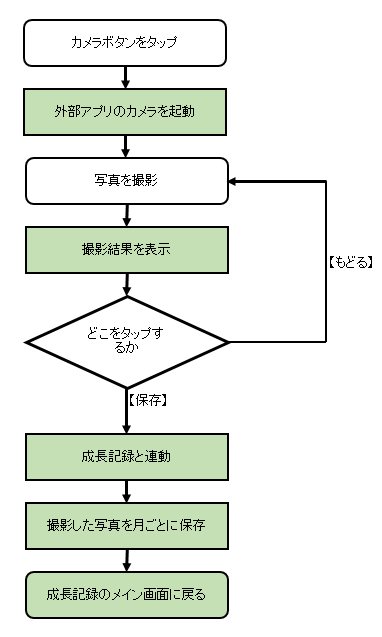
\includegraphics {camera.png}}
    \caption {カメラモジュールのフローチャート}
    \label{camera}
    \end{center}
\end{figure}

\subsubsection*{概要}
図\ref{camera}は、利用者が新しく写真を撮影する際のシステムの流れを示しています。

\subsubsection*{処理フロー}
\begin{itemize}
\item 外部アプリのカメラを起動し写真を撮影します。その後、【もどる】か【保存】を選択します。
\item 【もどる】をタップすることで写真を撮影する画面に遷移します。
\item 【保存】をタップすることで成長記録と連動します。その後、撮影した写真を月ごとに保存し成長記録のメイン画面(第\ref{grow}節)に遷移します。
\end{itemize}

\subsubsection{コメントモジュール\label{Coment}}
\begin{figure}[H]
    \begin{center}
    \resizebox{16.5cm}{!}{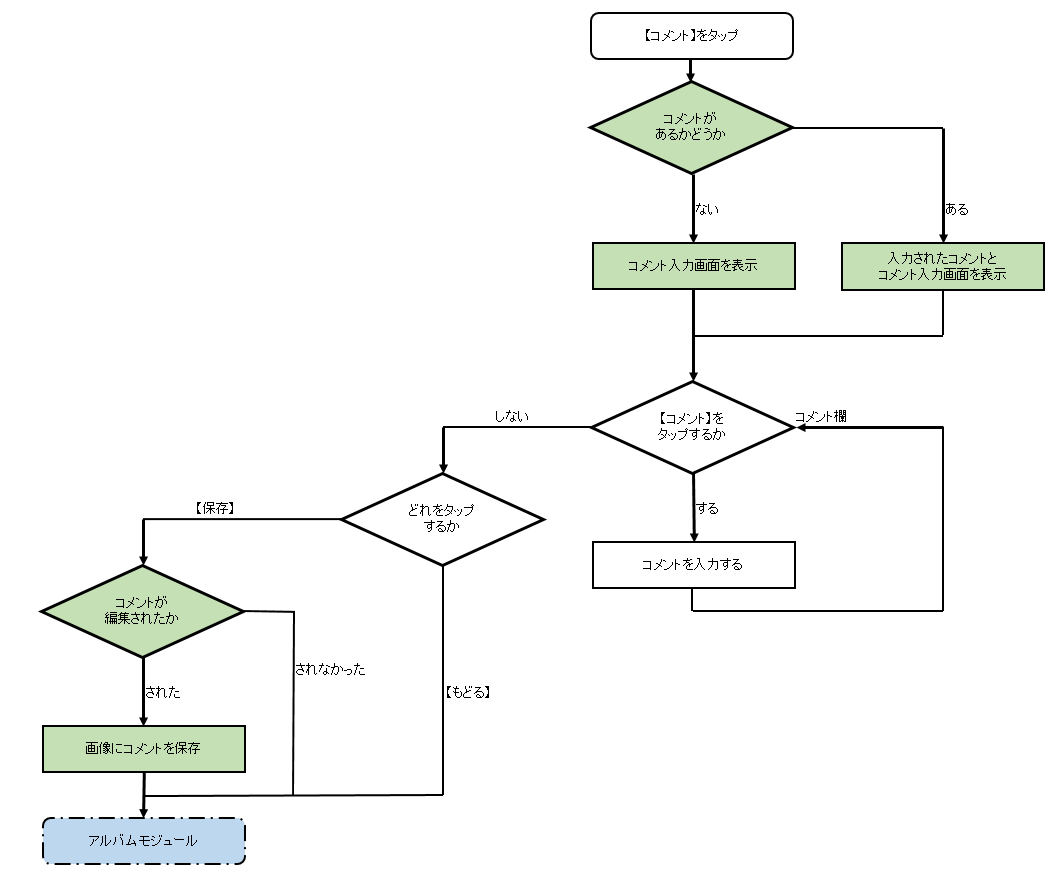
\includegraphics {coment.png}}
    \caption {コメントモジュールのフローチャート}
    \label{coment}
    \end{center}
\end{figure}

\subsubsection*{概要}
図\ref{coment}は、利用者が写真や記録にコメントを挿入・編集する際のシステムの流れを示しています。。

\subsubsection*{処理フロー}
\begin{itemize}
\item このモジュールに入ったときにその写真や記録にコメントが付与されているかを判定します。コメントがなければコメント入力画面のみ表示し、コメントがあればそのコメントとコメント入力画面を一緒に表示します。
\item コメント入力画面が表示されるとコメント欄をタップすることでコメントの書き込みが行えます。挿入、編集は何度でも行えます。
\item コメントの書き込みが終わった場合、もしくはコメントを書き込まなかった場合【保存】をタップするか、保存せずに【もどる】をタップするかを選択します。
\item 【保存】をタップした場合コメントの内容が変更されたかを判定し、変更されていれば内容を保存してアルバムモジュールに遷移します。変更されていなければ保存せずにアルバムモジュール(第\ref{Albam}節)に遷移します。
\item 【もどる】をタップすることで内容を保存せずアルバムモジュール(第\ref{Albam}節)に遷移します。
\end{itemize}
\newpage


\subsection{子育て窓口機能}
\subsubsection{子育て窓口モジュール\label{子育て窓口モジュール}} %ラベル名は「~モジュール」の「~」部分を使用。他の人が参照してくる場合もあるので(メイン画面は特に)

\begin{figure}[H]
    \begin{center}
      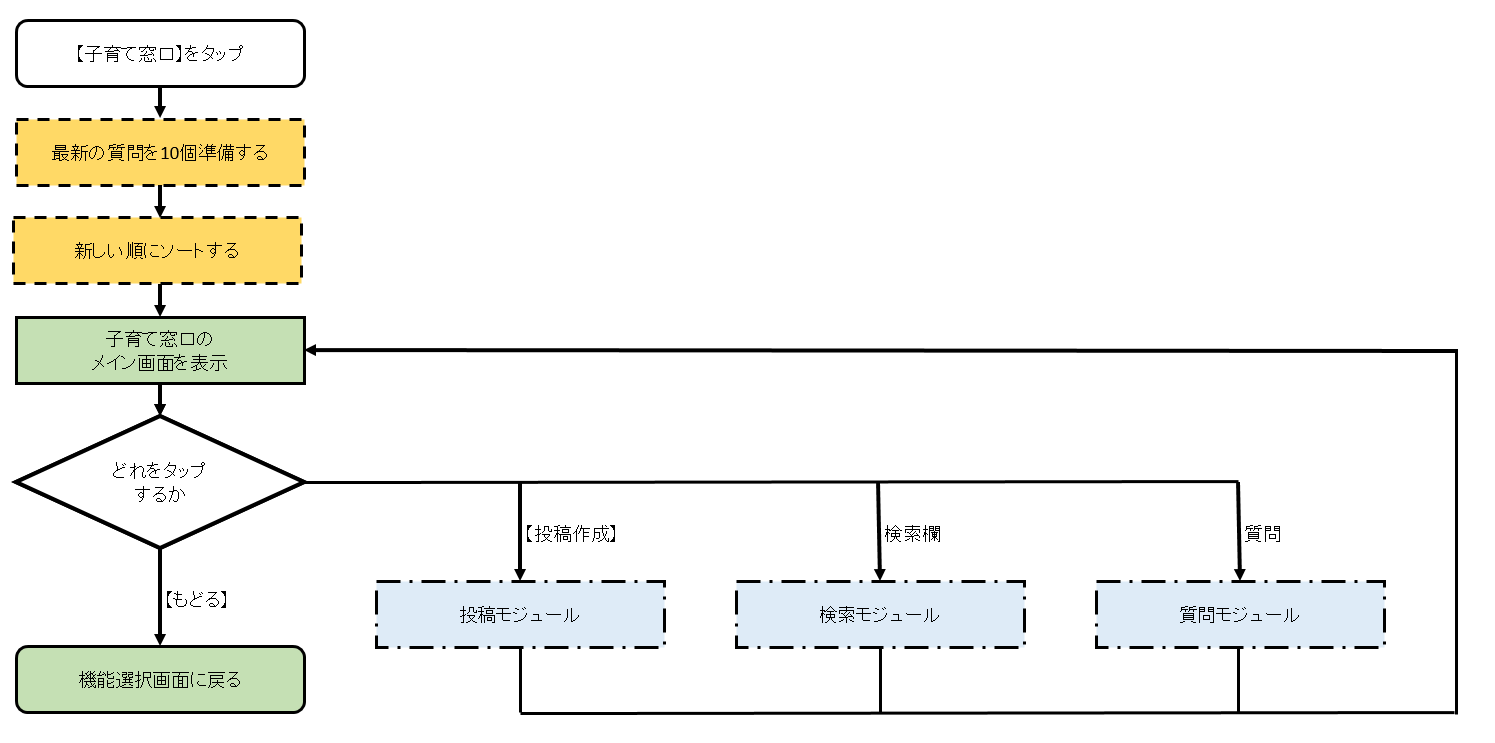
\includegraphics[height = 4.0cm]{子育て窓口_全体.png} %画像は各自で用意、大きさも自分で調整
    \caption {子育て窓口モジュールのフローチャート}
    \label{子育て窓口_全体}
    \end{center}
\end{figure}

\subsubsection*{概要}
図\ref{子育て窓口_全体}は、子育て窓口機能の各サブシステムを利用するまでのシステムの流れを示しています。
\subsubsection*{処理フロー}
\begin{itemize}
\item データベースに保存されている最新の質問10個を要求し、新しい順に画面に表示させます。
\item 【もどる】をタップすることで機能選択画面(第\ref{機能選択}節)に遷移します。
\item 【投稿作成】をタップすることで投稿モジュール(第\ref{投稿}節)を呼び出します。
\item 【検索】をタップすることで検索モジュール(第\ref{検索}節)を呼び出します。
\item 各質問をタップすることで質問モジュール(第\ref{質問}節)を呼び出します。

\end{itemize}

\subsubsection{投稿モジュール\label{投稿}} %ラベル名は「~モジュール」の「~」部分を使用。他の人が参照してくる場合もあるので(メイン画面は特に)
\begin{figure}[H]
    \begin{center}
      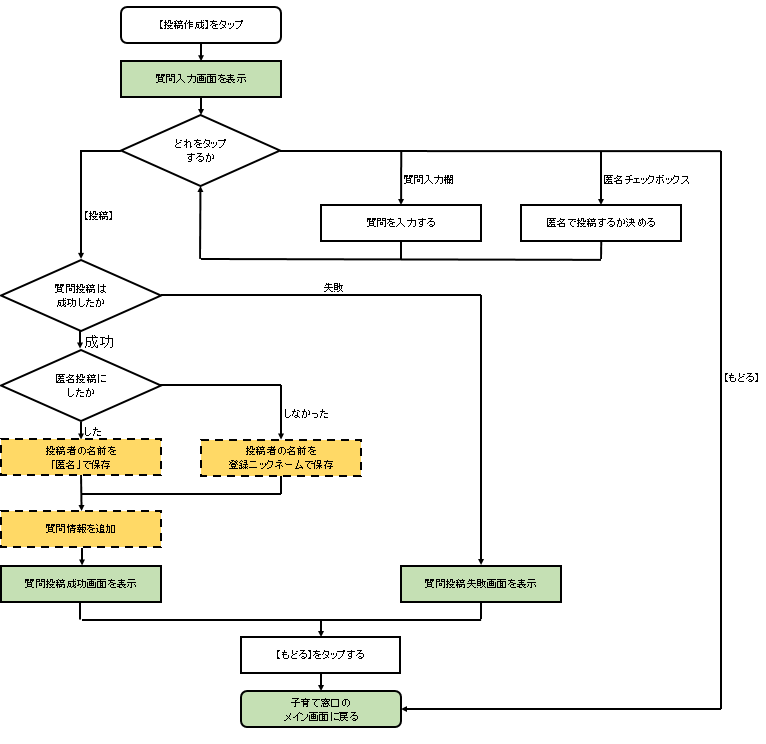
\includegraphics[height = 12.0cm] {子育て窓口_投稿.png} %画像は各自で用意、大きさも自分で調整
    \caption {投稿モジュールのフローチャート}
    \label{子育て窓口_投稿}
    \end{center}
\end{figure}
\subsubsection*{概要}
図\ref{子育て窓口_投稿}は、本システム利用者が子育てに関する質問を投稿する際のシステムの流れを示しています。
\subsubsection*{処理フロー}
\begin{itemize}
\item 質問入力欄をタップすることで質問を入力することができます。匿名で投稿するか、登録されているユーザ名で投稿するか決めることができ、匿名投稿をしたい場合は匿名チェックボックスをタップします。
\item 【投稿】をタップすることで投稿を行うことができます。
\item 投稿に失敗した場合は質問投稿失敗画面を表示させます。
\item 投稿に成功した場合はユーザ名と質問情報をデータベースに保存します。匿名チェックボックスをタップしていた場合は、ユーザ名を「匿名」で保存します。
\item 投稿に成功した場合は質問投稿成功画面を表示させます。
\item 投稿終了後、【もどる】をタップすることで子育て窓口機能のメイン画面(第\ref{子育て窓口}節)に遷移します。

\end{itemize}

\subsubsection{検索モジュール\label{検索}} %ラベル名は「~モジュール」の「~」部分を使用。他の人が参照してくる場合もあるので(メイン画面は特に)
\begin{figure}[H]
    \begin{center}
      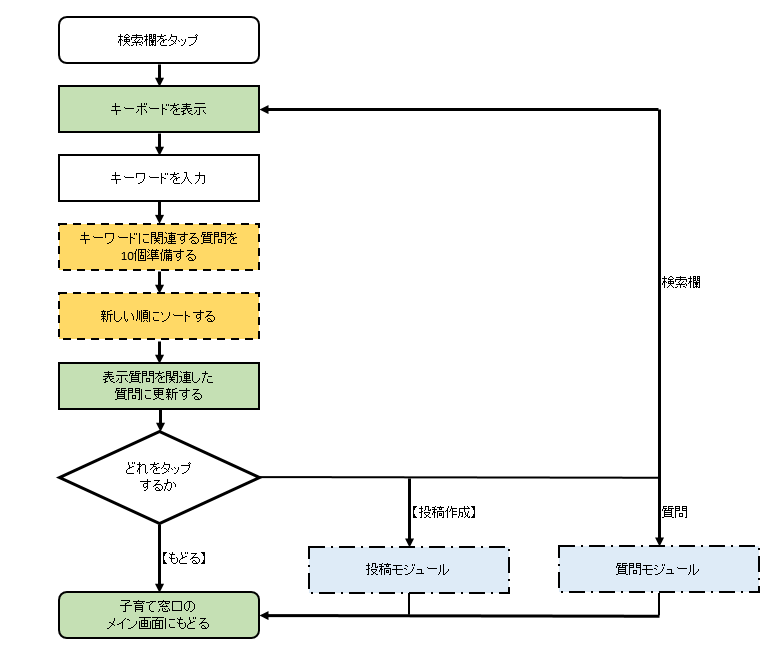
\includegraphics[height = 12.0cm] {子育て窓口_検索.png} %画像は各自で用意、大きさも自分で調整
    \caption {検索モジュールのフローチャート}
    \label{子育て窓口_検索}
    \end{center}
\end{figure}
\subsubsection*{概要}
図\ref{子育て窓口_検索}は、本システム利用者が子育てに関する質問をキーワードで検索し、キーワードに関連した質問を表示させる際のシステムの流れを示しています。
\subsubsection*{処理フロー}
\begin{itemize}
\item 検索欄をタップすることでキーボードが表示され、キーワードを入力することができます。入力されたキーワードに関連する質問10個をデータベースに要求し、新しい順に画面に表示させます。
\item 【もどる】をタップすることで子育て窓口機能のメイン画面(第\ref{子育て窓口}節)に遷移します。
\item 【投稿作成】をタップすることで投稿モジュール(第\ref{投稿}節)を呼び出します。
\item 各質問をタップすることで質問モジュール(第\ref{質問}節)を呼び出します。


\end{itemize}

\subsubsection{質問モジュール\label{質問}} %ラベル名は「~モジュール」の「~」部分を使用。他の人が参照してくる場合もあるので(メイン画面は特に)
\begin{figure}[H]
    \begin{center}
      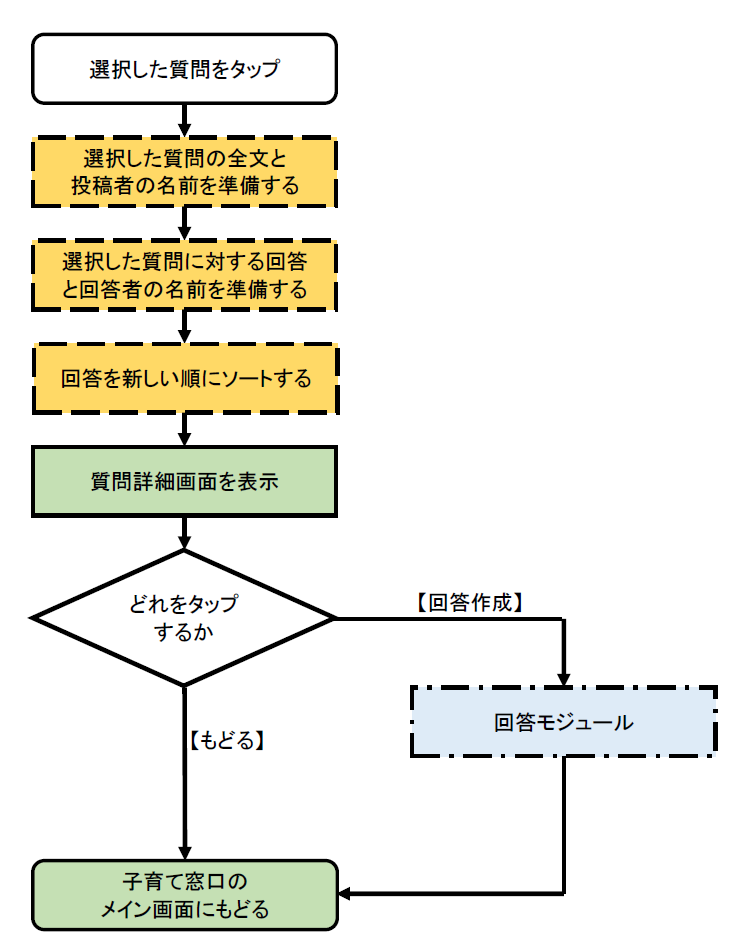
\includegraphics[height = 12.0cm] {子育て窓口_質問.png} %画像は各自で用意、大きさも自分で調整
    \caption {質問モジュールのフローチャート}
    \label{子育て窓口_質問}
    \end{center}
\end{figure}
\subsubsection*{概要}
図\ref{子育て窓口_質問}は、画面上に表示された各質問をタップした際のシステムの流れを示しています。
\subsubsection*{処理フロー}
\begin{itemize}
\item データベースに質問の全文と投稿者のユーザ名を要求し、画面に表示させます。
\item データベースに質問に対する回答の全文と回答者のユーザ名を要求し、画面に表示させます。
\item 【もどる】をタップすることで子育て窓口機能のメイン画面(第\ref{子育て窓口}節)に遷移します。
\item 【回答作成】をタップすることで回答モジュール(第\ref{回答}節)を呼び出します。

\end{itemize}

\subsubsection{回答モジュール\label{回答}} %ラベル名は「~モジュール」の「~」部分を使用。他の人が参照してくる場合もあるので(メイン画面は特に)
\begin{figure}[H]
    \begin{center}
      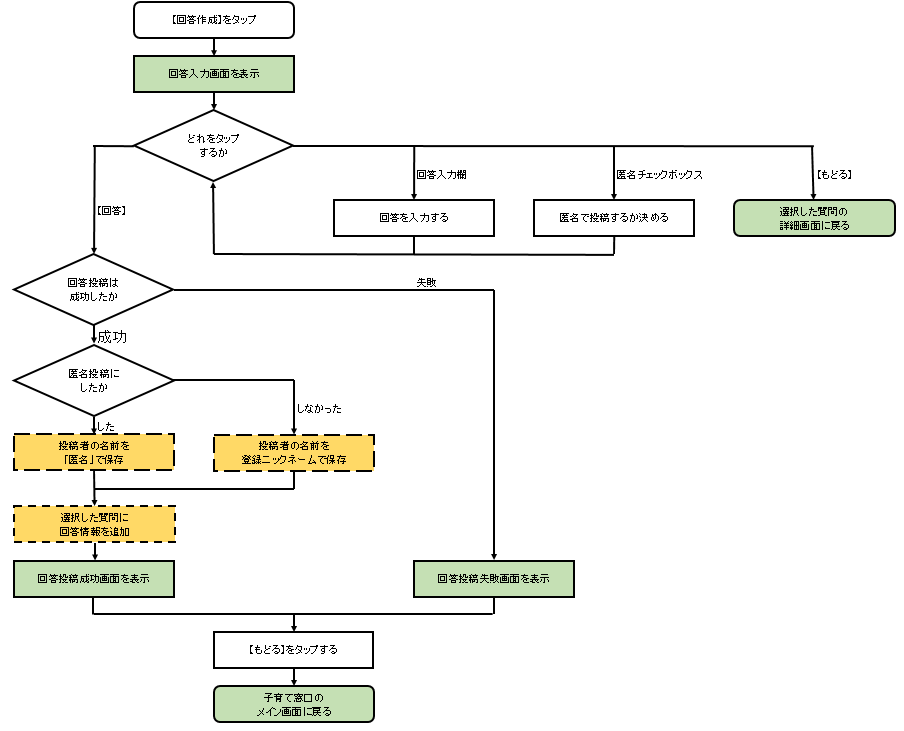
\includegraphics[height = 14.0cm] {子育て窓口_回答.png} %画像は各自で用意、大きさも自分で調整
    \caption {回答モジュールのフローチャート}
    \label{子育て窓口_回答} 
    \end{center} 
\end{figure}
\subsubsection*{概要}
図\ref{子育て窓口_回答}は、子育てに関する質問に対して回答を行う際のシステムの流れを示しています。
\subsubsection*{処理フロー}
\begin{itemize}
\item 回答入力欄をタップすることで回答を入力することができます。匿名で投稿するか、登録されているユーザ名で投稿するか決めることができ、匿名投稿をしたい場合は匿名チェックボックスをタップします。
\item 【回答】をタップすることで投稿を行うことができます。
\item 投稿に失敗した場合は回答投稿失敗画面を表示させます。
\item 投稿に成功した場合はユーザ名と回答情報をデータベースに保存します。匿名チェックボックスをタップしていた場合は、ユーザ名を「匿名」で保存します。
\item 投稿に成功した場合は回答投稿成功画面を表示させます。
\item 投稿終了後、【もどる】をタップすることで子育て窓口機能のメイン画面(第\ref{子育て窓口}節)に遷移します。

\end{itemize}

\newpage

\subsection{設定機能}
\subsubsection{設定モジュール\label{設定}} %ラベル名は「~モジュール」の「~」部分を使用。他の人が参照してくる場合もあるので(メイン画面は特に)
\begin{figure}[H]
    \begin{center}
      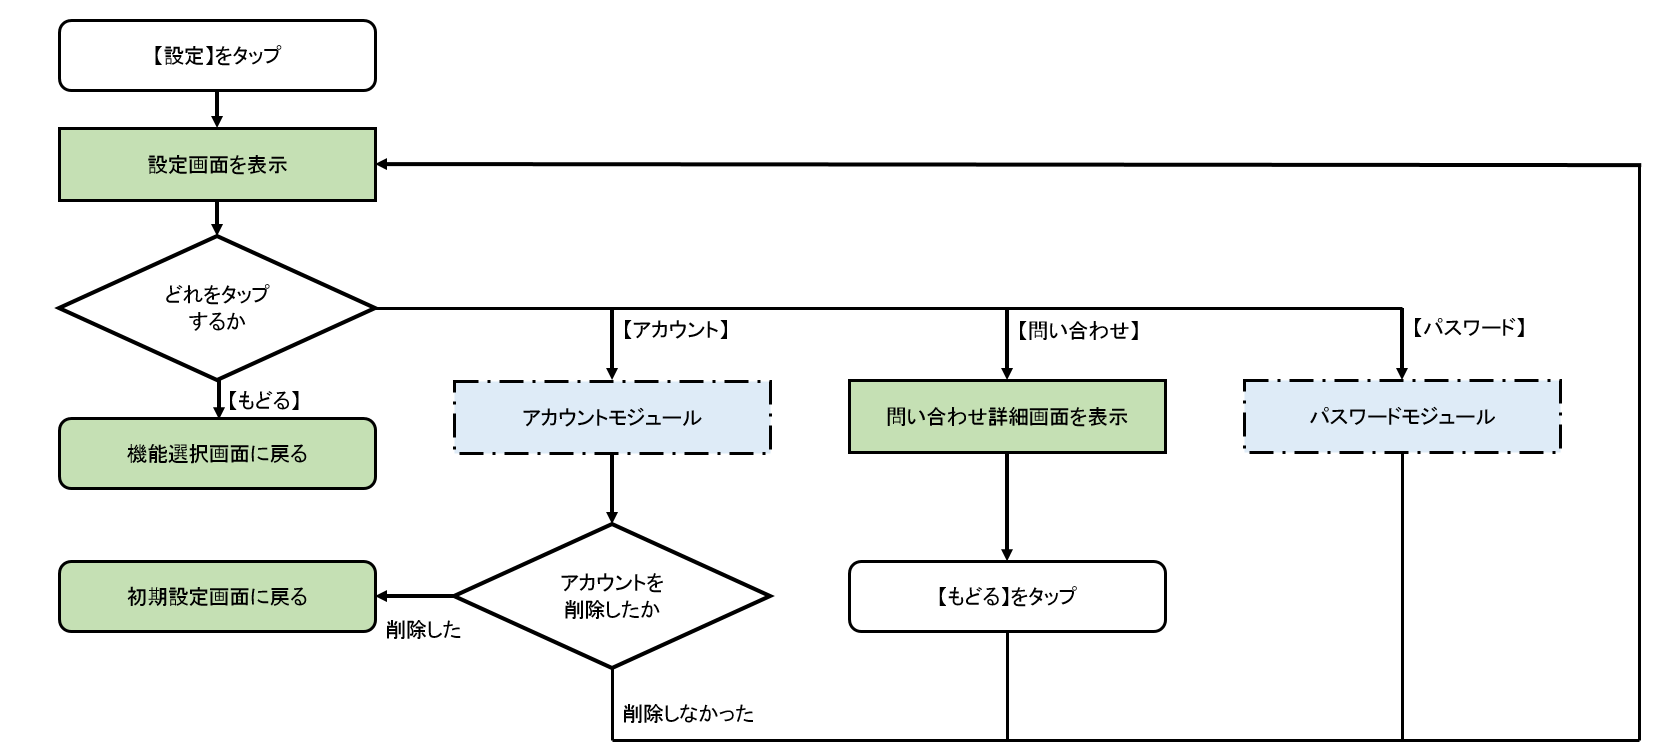
\includegraphics[height=8.0cm] {設定_全体.png} %画像は各自で用意、大きさも自分で調整
    \caption {設定モジュールのフローチャート}
    \label{設定_全体}
    \end{center}
\end{figure}
\subsubsection*{概要}
図\ref{設定_全体}は、設定機能の各サブシステムを利用するまでのシステムの流れを示しています。
\subsubsection*{処理フロー}
\begin{itemize}
\item 【アカウント】をタップすることでアカウントモジュール(第\ref{アカウント}節)を呼び出します。その後アカウントが削除されたかどうかで設定画面か初期設定画面(第\ref{初期設定}節)に遷移します。

\item 【問い合わせ】ボタンをタップすることで問い合わせ詳細画面を表示します。その後【もどる】ボタンをタップすることで設定画面(第\ref{設定}節)に遷移します。

\item 【パスワード】をタップすることでパスワードモジュール(第\ref{パスワード}節)を呼び出します。

\item 【もどる】をタップすることで機能選択画面(第\ref{機能選択}節)に遷移します。
\end{itemize}

\subsubsection{アカウントモジュール\label{アカウント}} %ラベル名は「~モジュール」の「~」部分を使用。他の人が参照してくる場合もあるので(メイン画面は特に)
\begin{figure}[H]
    \begin{center}
      \resizebox{16.5cm}{!}{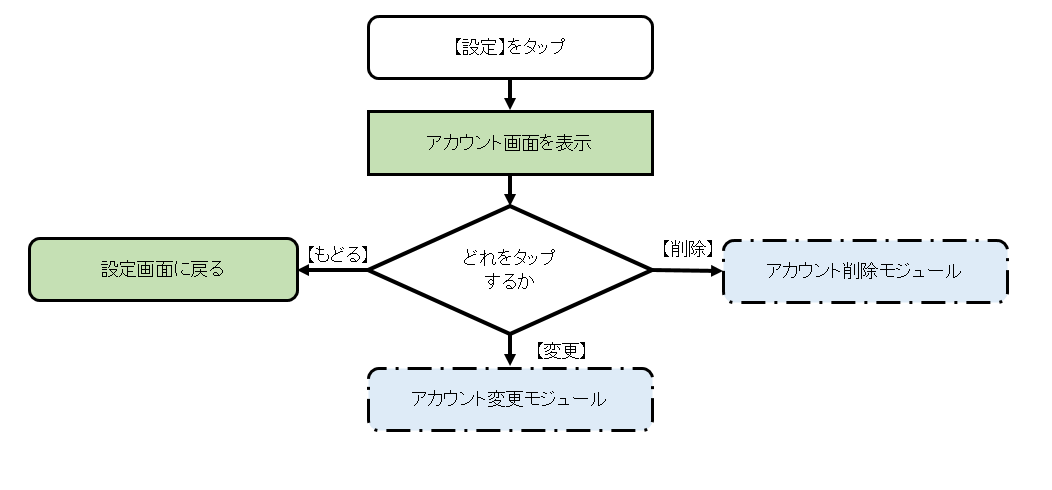
\includegraphics{設定_アカウント.png}} %画像は各自で用意、大きさも自分で調整
    \caption {アカウントモジュールのフローチャート}
    \label{設定_アカウント}
    \end{center}
\end{figure}
\subsubsection*{概要}
図\ref{設定_アカウント}は、子育て窓口機能を利用する際のアカウントの登録・変更・削除を行う際のシステムの流れを示しています。
\subsubsection*{処理フロー}
\begin{itemize}
\item 【変更】をタップすることでアカウント変更モジュール(第\ref{アカウント変更}節)を呼び出します。
\item 【削除】をタップすることでアカウント削除モジュール(第\ref{アカウント削除}節)を呼び出します。
\item 【もどる】をタップすることで設定画面(第\ref{設定}節)に遷移します。
\end{itemize}

\subsubsection{アカウント変更モジュール\label{アカウント変更}} %ラベル名は「~モジュール」の「~」部分を使用。他の人が参照してくる場合もあるので(メイン画面は特に)
\begin{figure}[H]
    \begin{center}
      \resizebox{16.5cm}{!}{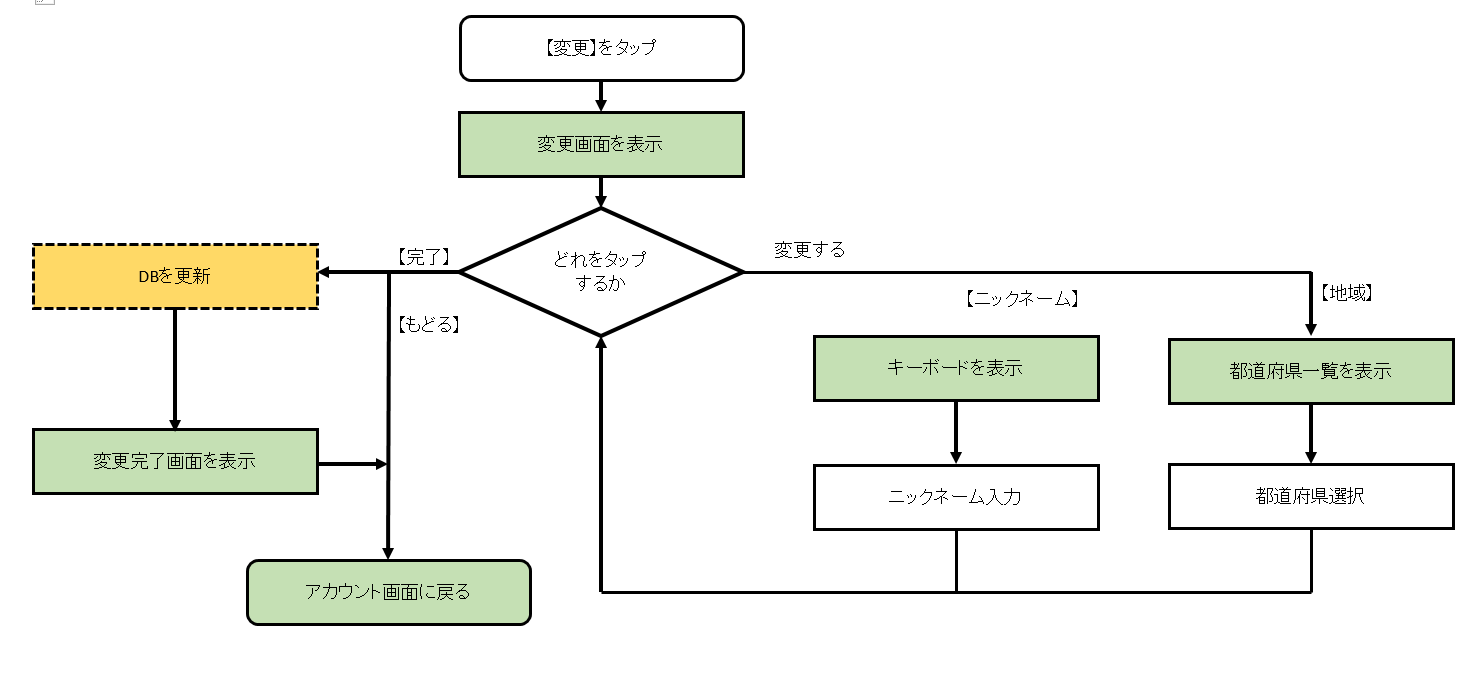
\includegraphics{設定_アカウント変更.png}}%画像は各自で用意、大きさも自分で調整
    \caption {アカウント変更モジュールのフローチャート}
    \label{設定_アカウント変更}
    \end{center}
\end{figure}
\subsubsection*{概要}
図\ref{設定_アカウント変更}は、アカウントの変更を行う際のシステムの流れを示しています。
\subsubsection*{処理フロー}
\begin{itemize}
\item 【ニックネーム】をタップすることで画面下にキーボードが表示され、名前入力を行いニックネームの変更が可能になります。
\item 【地域】をタップすることで47都道府県をタップして選択できるドロップダウンリストを【都道府県コード順」に表示させ、住んでいる地域設定を行い地域の変更が可能になります。
\item 【完了】をタップした場合【ニックネーム】と【地域】の設定が正しく行われていればデータベースを更新しアカウントの変更を行います。
\item 【もどる】ボタンをタップすることでアカウント画面(第\ref{アカウント}節)に遷移します。
\end{itemize}

\subsubsection{アカウント削除モジュール\label{アカウント削除}} %ラベル名は「~モジュール」の「~」部分を使用。他の人が参照してくる場合もあるので(メイン画面は特に)
\begin{figure}[H]
    \begin{center}
      \resizebox{16.5cm}{!}{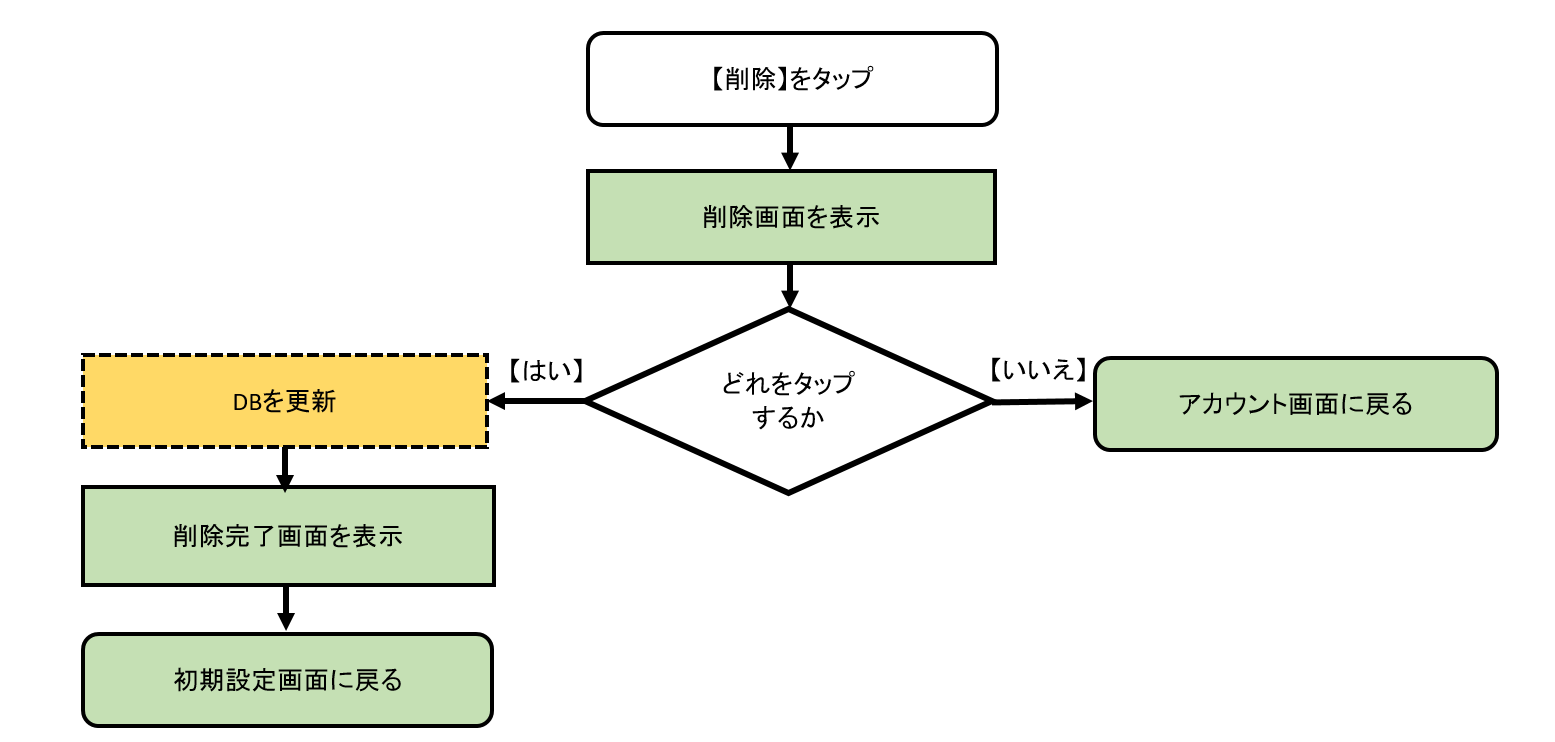
\includegraphics{設定_アカウント削除.png}} %画像は各自で用意、大きさも自分で調整
    \caption {アカウント削除モジュールのフローチャート}
    \label{設定_アカウント削除}
    \end{center}
\end{figure}
\subsubsection*{概要}
	図\ref{設定_アカウント削除}は、アカウントの削除を行う際のシステムの流れを示しています。
\subsubsection*{処理フロー}
\begin{itemize}
\item 【はい】をタップすることでデータベースを更新しアカウントの削除を行います。その後削除完了画面を表示し初期設定画面(第\ref{初期設定}節)に遷移します。
\item 【いいえ】をタップすることでアカウント画面(第\ref{アカウント}節)に遷移します。
\end{itemize}

\subsubsection{パスワードモジュール\label{パスワード}} %ラベル名は「~モジュール」の「~」部分を使用。他の人が参照してくる場合もあるので(メイン画面は特に)
\begin{figure}[H]
    \begin{center}
       \resizebox{16.5cm}{!}{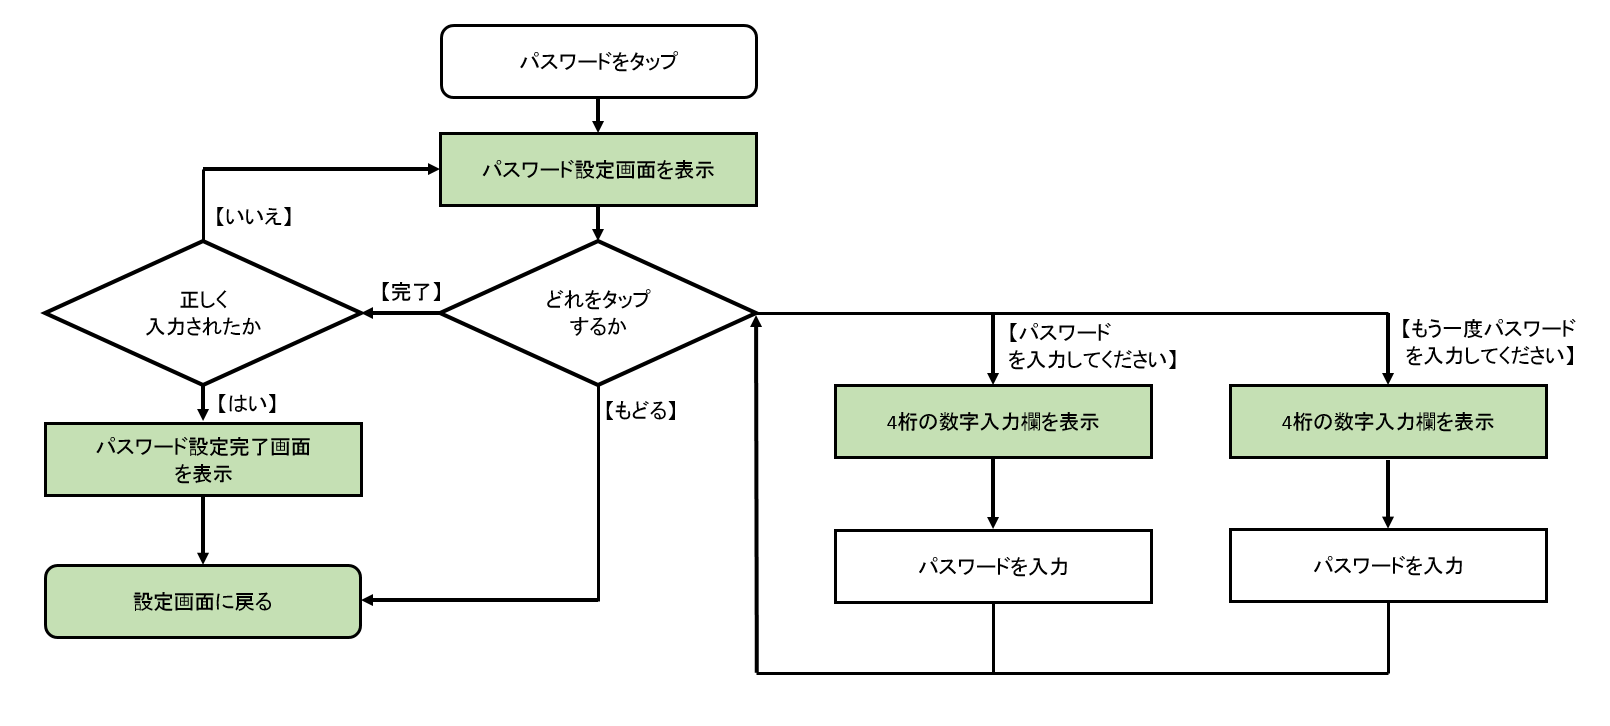
\includegraphics{設定_パスワード.png}}%画像は各自で用意、大きさも自分で調整
    \caption {パスワードモジュールのフローチャート}
    \label{設定_パスワード}
    \end{center}
\end{figure}
\subsubsection*{概要}
図\ref{設定_パスワード}は、こどもがゲーム機能を利用する際に他の機能や他のシステムを利用できないようにパスワードを設定する際のシステムの流れを示しています。
\subsubsection*{処理フロー}
\begin{itemize}
\item 【パスワードを入力してください】をタップし4桁の数字を入力することでパスワードの設定を行います。
\item【もう一度パスワードを入力してください】をタップし4桁のパスワードを入力することでパスワードの確認を行います。
\item 【完了】をタップした場合パスワードが正しく入力されていればパスワード設定画面完了画面を表示し設定画面(第\ref{設定}節)に遷移します。正しく入力されていなければパスワード設定画面(本節)に遷移します。
\item 【もどる】をタップすることで設定画面(第\ref{設定}節)に遷移します。
\end{itemize}

\newpage

\section{データベース設計}
本章では、システムで用いるデータベースの設計について記します。
\subsection{データテーブル相関図}
本小節では、テーブル間の関係性をER図を用いて示します。
\begin{figure}[H]
  \begin{center} %センタリングする
    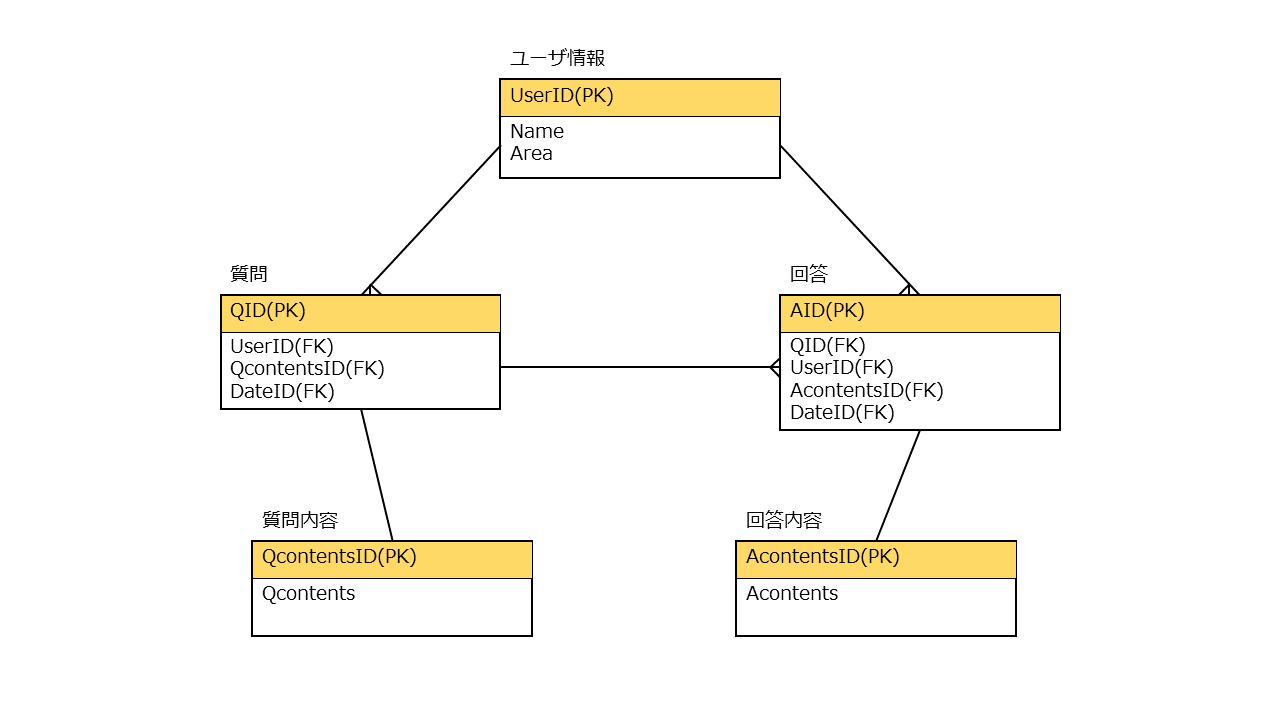
\includegraphics[width=16.0cm]{ER図v2.png}
    \caption{データテーブルER図} %タイトルをつける
    \label{fig:er} %ラベルをつけ図の参照を可能にする
  \end{center}
\end{figure}

今回用いるデータベースシステムでは、ユーザ情報の定義と質問箱の管理を行っています。\\
図\ref{fig:er}のように、親ユーザと質問・回答の関係性、質問と回答の関係性はそれぞれ1対多の関係性になっており、それ以外のテーブルは1対1の関係性となっています。

%ユーザ情報 -> アカウント情報に変えたほうがいい??????
\subsection{データテーブル設計}
本小節では、それぞれのデータテーブルの詳細について記します。

\subsubsection{ユーザ情報テーブル}

\begin{table}[H]
    \caption{ユーザ情報}
    \label{tbl: user}
    \begin{center}
        \begin{tabular}{|c|c|c|c|c|c|} \hline
            属性 & データ型 & データ長 & SQLite & key:Table名 & NULL\\ \hline \hline
            UserID & 半角英数字型 & 6文字固定長 & TEXT & PK & Not\\ \hline
            Name & 全角文字型 & 10文字可変長 & TEXT & & Not\\ \hline
            Area & 全角文字型 & 5文字可変長 & TEXT & & Not\\ \hline
        \end{tabular}
    \end{center}
\end{table}

表\ref{tbl: user}ではユーザ情報を格納しています。ユーザIDと名前、住んでいる地域を管理することで、質問箱でどの地域の人が投稿を行っているのか分かるようにしています。\\
各フィールドの概要は以下の通りです。
\begin{itemize}
  \item ユーザID(UserID):
  ユーザテーブルの主キー
  \item ユーザ名(Name):
  ユーザの名前
  \item 居住地域名(Area):
  ユーザが住んでいる地域名
\end{itemize}

\subsubsection{質問テーブル}

\begin{table}[H]
    \caption{質問}
    \label{tbl: question}
    \begin{center}
        \begin{tabular}{|c|c|c|c|c|c|} \hline
            属性 & データ型 & データ長 & SQLite & key:Table名 & NULL\\ \hline \hline
            QID & 半角英数字型 & 8文字固定長 & TEXT & PK & Not\\ \hline
            UserID & 半角英数字型 & 6文字固定長 & TEXT & FK:親ユーザー情報 & Not\\ \hline
            QcontentsID & 半角英数字型 & 10文字固定長 & TEXT & FK:質問内容 & Not\\ \hline
            Date & 日付型 & 20文字固定長 & NUMERIC & & Not\\ \hline
        \end{tabular}
    \end{center}
\end{table}

表\ref{tbl: question}では、質問と質問者の関連付けを行っています。質問IDを主キーとし、ユーザ情報テーブル、質問内容テーブルといったテーブルの主キーを外部キーとすることで、質問を投稿、確認できるようにしています。\\
各フィールドの概要は以下の通りです。
\begin{itemize}
  \item 質問ID(QID):
  質問テーブルの主キー
  \item ユーザID(UserID):
  ユーザテーブルの主キー
  \item 質問内容ID(QcontentsID):
  質問内容テーブルの主キー
  \item 日付(Date):
  投稿した日付と時刻の保存
\end{itemize}

\subsubsection{回答テーブル}
\begin{table}[H]
    \caption{回答}
    \label{tbl: answer}
    \begin{center}
        \begin{tabular}{|c|c|c|c|c|c|} \hline
            属性 & データ型 & データ長 & SQLite & key:Table名 & NULL\\ \hline \hline
            AID & 半角英数字型 & 8文字固定長 & TEXT & PK & Not\\ \hline
            QID & 半角英数字型 & 8文字固定長 & TEXT & FK:質問 & Not\\ \hline
            UserID & 半角英数字型 & 6文字固定長 & TEXT & FK:親ユーザー情報 & Not\\ \hline
            AcontentsID & 半角英数字型 & 10文字固定長 & TEXT & FK:回答内容 & Not\\ \hline
            Date & 日付型 & 20文字固定長 & NUMERIC & & Not\\ \hline
        \end{tabular}
    \end{center}
\end{table}
表\ref{tbl: answer}では、回答と回答者の関連付けを行っています。回答IDを主キーとし、質問テーブルと同様に外部キーを指定しています。また、質問テーブルも外部キーとしています。これにより、一つの質問に対して、複数の回答を関連付けることができます。\\
各フィールドの概要は以下の通りです。
\begin{itemize}
  \item 回答ID(AID):
  回答テーブルの主キー
  \item 質問ID(QID):
  質問テーブルの主キー
  \item ユーザID(UserID):
  ユーザテーブルの主キー
  \item 回答内容ID(AcontentsID):
  回答内容テーブルの主キー
  \item 日付(Date):
  投稿した日付と時刻の保存
\end{itemize}

\subsubsection{質問内容テーブル}
\begin{table}[H]
    \caption{質問内容}
    \label{tbl: qcontents}
    \begin{center}
        \begin{tabular}{|c|c|c|c|c|c|} \hline
           属性 & データ型 & データ長 & SQLite & key:Table名 & NULL\\ \hline \hline
            QcontentsID & 半角英数字型 & 10文字固定長 & TEXT & PK & Not\\ \hline
            Qcontents & 全角文字型 & 1000文字可変長 & TEXT & & Not\\ \hline
        \end{tabular}
    \end{center}
\end{table}
表\ref{tbl: qcontents}では、質問内容を管理を行っています。質問内容の本文は全角文字型で1000文字まで投稿することができます。質問内容と質問を分けて管理することで、データの正規化を図っています。\\
各フィールドの概要は以下の通りです。
\begin{itemize}
  \item 質問内容ID(QcontentsID):
  質問内容テーブルの主キー
  \item 質問内容(Qcontents):
  質問内容の本文
\end{itemize}

\subsubsection{回答内容テーブル}
\begin{table}[H]
    \caption{回答内容}
    \label{tbl: acontents}
    \begin{center}
        \begin{tabular}{|c|c|c|c|c|c|} \hline
            属性 & データ型 & データ長 & SQLite & key:Table名 & NULL\\ \hline \hline
            AcontentsID & 半角英数字型 & 10文字固定長 & TEXT & PK & Not\\ \hline
            Acontents & 全角文字型 & 1000文字可変長 & TEXT & & Not\\ \hline
        \end{tabular}
    \end{center}
\end{table}
表\ref{tbl: acontents}では回答内容を管理を行っています。質問内容テーブルと同様に、回答内容の本文も全角文字型で1000文字まで投稿できます。\\
各フィールドの概要は以下の通りです。
\begin{itemize}
  \item 回答内容ID(AcontentsID):
  回答内容テーブルの主キー
  \item 回答内容(Acontents):
  回答内容の本文
\end{itemize}



\end{document}
